%-II - 10
\chapter{Postulats de quantification de Feynman}

\hfill (R.P. Feynman, Fev. Mod. Phys. 20, 2, 1948, p. 367)

\vspace{.5cm}
Dans ce chapitre II, on énonce de façon précise les postulats de Feynman
(\S A). On les applique ensuite, d'abord au cas simple d'une particule libre
(\S B); puis, après avoir défini la fonction d'onde (\S ch au cas d'une particule dens un potentiel V(x), ce qui permet d'obtenir l'équation de Schrödinger .
(\S D) et de prouver ainsi l'équivalence entre la nouvelle formulation de la
mécanique quantique et les précédentes.

\section{Enoncé des postulats}

Les postulats de Feynman permettent de calculer la quantité
< x''t'' | x't' > qui représente l'amplitude de probabilité pour que la
particule, au point x' à l'instant t', se trouve au point x'' à l'instant
t''.

Avant d'énoncer les postulats, voyons comment cette amplitude
se présente dans la formulation usuelle de la mécanique quantique :

\subsection{Etude de < x''t'' | x't' >}

\subsubsection{dans le point de vue de Schrödinger}

Rappelons que dans le point de vue de Schrödinger, les vecteurs
d'état qui représentent le système physique, | $\psi$(t) > dépendent du temps.
Les observables, A, par contre, sont indépendantes du temps, ainsi, bien
entendu, que leurs états propres. Par exemple, X étant l'observable représentant
la position de la particule, on a l'équation aux valeurs propres,
indépendante du temps X | x > $=$ x | x >.

Dans la représentation X, le vecteur | $\psi$(t) > est représenté
par sa fonction d'onde

< x | $\psi$(t) > $=$ $\psi$(x,t).

L'évolution du vecteur d'état | $\psi$(t) > peut être décrite à l'aide
de l'opérateur d'évolution U(t'',t') qui est unitaire (conséquence du fait
que La translation dans le temps est une opération de symétrie) :

| $\psi$(t'') > $=$ U(t'',t') | $\psi$(t') >

Dans ce formalisme, l'amplitude de probabilité s'écrit :

< x''t'' | x't' > $=$ < x'' | U(t'', t') | x' >

% 11
Remarque : < x'' | U(t'',t') | x' > représente la fonction de Green
de l'équation de Schrödinger : c'est la valeur au point x'' à l'instant t''
de la solution de l'équation de Schrödinger qui se réduit à l'instant
t $=$ t' à une fonction de Dirac au point x', $\delta$(x - x'). On appelle
< x''t'' | x't' > également le “propagateur'' de l'équation de Schrödinger.

\subsubsection{dans le point de vue de Heisenberg}

Rappelons que dans le point de vue de Heisenberg, les vecteurs
d'état | $\psi$ >, sont indépendants du temps. Les observables, et en conséquence,
les états propres de ces observables dépendent au contraire du
temps : l'équation aux valeurs propres de l'observable X(t) s'écrit :

X(t) | x,t > $=$ x | x,t >.

A l'instant t, le vecteur | $\psi$ > peut être représenté par sa projection
sur la base complète | x,t > : on obtient la fonction d'onde
< x,t | $\psi$ > $=$ $\psi$(x,t).

Il est évident que ce point de vue est équivalent à celui de
Schrödinger : seul le mouvement relatif du vecteur d'état et des vecteurs
de base des observables a une signification physique et ce mouvement
relatif est le même dans les deux points de vue.

Quelle est, dans ce formalisme, l'amplitude de probabilité pour
que la particule, en x' à l'instant t', se trouve en x'' à l'instant t'' ?
Le vecteur d'état | $\psi$ >, indépendant du temps, doit être vecteur propre
de X(t') correspondant à la valeur propre x'. | $\psi$ > est donc confondu
avec | x',t' >. L'amplitude de probabilité cherchée est égale à la projection
de | $\psi$ > sur l'état propre de l'opérateur X(t''), de valeur rropre
x'', que nous avons désigné par | x'',t'' >. Elle est donc égale à
| x'',t'' | $\psi$ > $=$ < x'',t'' | x',t' >.

Nous voyons donc que la notation que nous avons adoptée a
priori pour cette amplitude est celle du point de vue de Heisenberg.

 
%-12
\subsection{Les postulats de Feynman}

{\bf Postulat I} : < x''t'' | x't' > est constitué par une somme de contributions,
une pour chaque chemin d'espace-temps reliant (x't') à (x'' t'').

La notion de sommation sur chaque chemin d'espace-temps est
ambigüe et pose des problèmes d'analyse fonctionnelle délicats,
Feynman précise cette notion de la façon suivante.

Au lieu de se définir un chemin par la donnée d'une fonction
continue x(t) entre (x't') et (x''t''), on divise l'intervalle t't'' en
n intervalles égaux $\epsilon$ par (n-1) temps intermédiaires t$_\mt{i}$,
t$_\mt{i+1}$, ... et
on définit un chemin par la donnée de la suite double

\begin{center}
t' t$_1$ t$_2$ ... t$_\mt{i}$ t$_\mt{i+1}$ ... t$_\mt{n-1}$ t''

x' x$_1$ x$_2$ ... x$_\mt{i}$ x$_\mt{i+1}$ ... x$_\mt{n-1}$ x''
\end{center}

que l'on note encore
\begin{center}
M' M$_1$ M$_2$ ... M$_\mt{i}$ M$_\mt{i+1}$ ... M$_\mt{n-1}$ M''
\end{center}

On fait ensuite tendre $\epsilon$ vers zéro (ou encore n $=$ (t''-t')/$\epsilon$
vers l'infini).

Cependant, aussi petit que soit $\epsilon$, la donnée d'une suite des M
ne suffit pas à déterminer le chemin continu x(t) :

\begin{center} 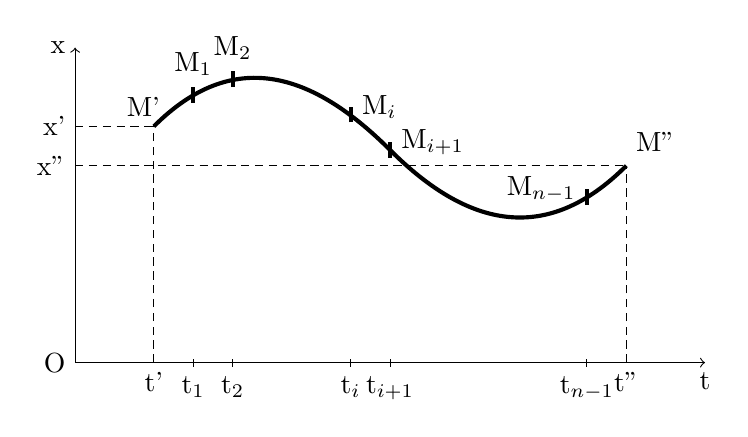
\begin{tikzpicture}
% axes
\draw [->] (0,0) --++ (8,0) node [below] {t};
\draw [->] (0,0) --++ (0,4) node [left] {x};
\node at (0,0) [left]{O};
% coordonnées et points
\draw [densely dashed] (0,3) node [left] {x'} --++ (1,0);
\draw [densely dashed] (1,0) node [below] {t'} --++ (0,3);
\node at (1.2,3) [above left]{M'};
\draw [densely dashed] (0,2.5) node [left] {x''} --++ (7,0);
\draw [densely dashed] (7,0) node [below] {t''} --++ (0,2.5);
\node at (7,2.8) [right]{M''};
% intermédiaires
\draw (1.5,-0.05) node [below] {t$_1$} --++ (0,0.1);
\draw [line width=1.5pt] (1.5,3.3) --++ (0,0.2) node [above]{M$_1$};
\draw (2,-0.05) node [below] {t$_2$} --++ (0,0.1);
\draw [line width=1.5pt] (2,3.5) --++ (0,0.2) node [above]{M$_2$};
% intermédiaires fin
\draw (6.5,-0.05) node [below] {t$_{\mt{n}-1}$} --++ (0,0.1);
\draw [line width=1.5pt] (6.5,2) --++ (0,0.2) node [left]{M$_{\mt{n}-1}$};
% intermédiaires milieu
\draw (3.5,-0.05) node [below] {t$_\mt{i}$} --++ (0,0.1);
\draw [line width=1.5pt] (3.5,3.05) --++ (0,0.2) node [right]{M$_\mt{i}$};
\draw (4,-0.05) node [below] {t$_{\mt{i}+1}$} --++ (0,0.1);
\draw [line width=1.5pt] (4,2.6) --++ (0,0.2) node [right]{M$_{\mt{i}+1}$};
% Chemin
\draw [line width=1.5pt] (1,3) .. controls (2,4) and (3,3.7) .. (4,2.7);
\draw [line width=1.5pt] (4,2.7) .. controls (5,1.7) and (6,1.5) .. (7,2.5);
\end{tikzpicture} \end{center}
%-13—

Feynman définit le chemin de façon complète en postulant qu'il
faut joindre deux points consécutifs M$_\mt{i}$ et M$_\mt{i+1}$ par le
chemin classique
qui passe par ces deux points (si le Lagrangien du mouvement ne dépend
que de x et $\dot{\mt{x}}$ et non des dérivées supérieures, les équations de
Lagrange
sont du second ordre, et la donnée des deux points M$_\mt{i}$ et
M$_\mt{i+1}$ suffit à définir le chemin classique).

Grâce à cette définition complète du chemin, nous avons pu,
pour chaque valeur de $\epsilon$ (donc de n), paramétrer, à l'aide des
x$_\mt{i}$, l'ensemble des chemins. La sommation sur les chemins revient
alors à intégrer
sur les paramètres x$_\mt{i}$ et on peut écrire :

\begin{center}
(1) \ \ \ < x''t'' | x't' > $=$ 
$\lim_{\,\epsilon \to \,0}$ $\int$ .. $\int$
dx$_1$ .. dx$_\mt{i}$ .. dx$_\mt{n-1}$
$\phi$(x',x$_1$ .. x$_\mt{i}$ .. x$_\mt{n-1}$,x'')
\end{center}

$\phi$(x',x$_1$ .. x$_\mt{i}$ .. x$_\mt{n-1}$,x'') représente la contribution d'un chemin tel
qu'il a été défini plus haut. le second postulat nous fournira la valeur
de $\phi$.

Remarque : Le fait que < x''t'' | x't' > est une somme de contributions est
en fait une conséquence du principe général de superposition.

X(t) étant une observable, nous avons en effet la relation de
fermeture

\begin{center}
$\int$ | x t > < x t | dx $=$ 1
\end{center}

En injectant les relations de fermeture relatives aux instants
t$_1$, .. t$_\mt{i}$, .. t$_\mt{n-1}$, nous obtenons :


\begin{center}
< x''t'' | x't' > $=$ $\int$ .. $\int$ dx$_1$ .. dx$_\mt{i}$ .. dx$_\mt{n-1}$
< x''t'' | x$_1$t$_1$ > < x$_1$t$_1$ | ... | x$_\mt{n-1}$t$_\mt{n-1}$ > < x$_\mt{n-1}$t$_\mt{n-1}$ | x''t'' >
\end{center}

%  14

{\bf Postulat II} : La contribution de chacun des chemins définis plus haut est
(à un facteur de normalisation près, N, qui est le même pour tous les
chemins) égale à exp $\frac{\mt{i}}{\hbar}$ S, S étant l'action classique calculée le long
du chemin.

Remarquons tout d'abord que $\hbar$ a les dimensions d'une action
et que $\frac{\mt{S}}{\hbar}$ est bien, de ce fait, sans dimensions.

D'autre part, d'après la définition du chemin que nous avons
donnée dans le postulat I

\[
\mt{S} = \sum_{\mt{i}=0}^{\mt{n}-1} \mt{S} (\mt{x}_\mt{i}, \mt{x}_\mt{i+1})
 \ \ \ \ \ \ \ \ \ (\mt{en posant }\mt{x}_0 = \mt{x'})
\]

S (x$_\mt{i}$, x$_\mt{i+1}$) représentant l'action prise le long du chemin suivi par
une particule classique entre M$_\mt{i}$ et M$_\mt{i+1}$ c'est-à-dire encore

\[
\mt{S} (\mt{x}_\mt{i}, \mt{x}_\mt{i+1}) = \mt{min } \int_{\mt{t}_\mt{i}}^{\mt{t}_\mt{i+1}}
\mc{L} [ \mt{x(t)}, \dot{\mt{x}}\mt{(t)} ] \mt{dt}
\]
Nous pouvons alors écrire :
\[
\mt{(2)\ \ \ < x''t'' | x't' > } = \lim_{\,\epsilon \to \,0} \mt{N} \int...\int
\mt{dx}_1..\mt{dx}_\mt{i}..\mt{dx}_\mt{n-1} \exp\frac{\mt{i}}{\hbar}
\sum_{\mt{i}=0}^{\mt{n}-1} \mt{S} (\mt{x}_\mt{i}, \mt{x}_\mt{i+1})
\]

C'est cette relation fondamentale qui nous servira par la suite.

{\bf Remarques :}

a) Quelle est la dimension de N ?

< x''t'' | x't' > a pour dimension L$^{-1}$. En effet, pour t'' $=$ t'',
l'amplitude se réduit à < x'' | x' > $= \delta$  (x'' - x'). Or la fonction
$\delta$ a pour dimension l'inverse d'une longueur (d'après la relation
fondamentale $\int \delta$(x)dx $=1$). L'intégrale de l'expression de < x''t'' | x't' > 
a pour dimension L$^{n-1}$. N a donc la dimension L$^{-n}$ et nous écrivons
\[
\mt{N}=\frac{1}{\mt{A}^\mt{n}}
\ \ \ \ \ \ \ \ \ \ \ \mt{(A ayant les dimensions d'une longueur).}
\]
 
%-15
b) Que se passe-t-il à la limite classique ($\hbar \to 0$)?

Les seuls chemins dont les contributions ne se détruisent pas par
interférence sont ceux qui correspondent à l'action stationnaire
par rapport à la variation des x$_\mt{i}$ c'est-à-dire les chemins classiques
du principe de Hamilton (cf Introduction).

Nous allons maintenant appliquer les postulats de Feynman au
calcul du propagateur dans un cas simple : celui de la particule libre.

\section{Calcul effectif de < x''t'' | x't' > pour la particule libre}

\subsection{Expression de S(x$_\mt{i}$, x$_\mt{i+1}$)}

Pour la particule libre, le chemin classique entre M$_\mt{i}$ et M$_\mt{i+1}$
est la ligne droite. La vitesse v est constante et égale à
(x$_\mt{i+1}$ - x$_\mt{i}$)/$\epsilon$

\[
\mt{S}(\mt{x}_\mt{i}, \mt{x}_\mt{i+1}) = \int_{\mt{t}_\mt{i}}^{\mt{t}_\mt{i+1}}
\frac{1}{2}\mt{mv}^2 = \frac{1}{2}\mt{mv}^2 \epsilon
 = \frac{\mt{m}}{2\epsilon}(\mt{x}_\mt{i+1}-\mt{x}_\mt{i})^2
\]
On a donc :
\[
\mt{(3)\ \ \ < x''t'' | x't' > } = \lim_{\,\epsilon \to \,0} \mt{A}^{-\mt{n}}
\int...\int
\exp\frac{\mt{im}}{2\hbar\epsilon}
[(\mt{x}_1-\mt{x'})^2 + (\mt{x}_2-\mt{x}_1)^2 +..+ (\mt{x'' }-\mt{x}_\mt{n-1})^2]
\mt{dx}_1...\mt{dx}_\mt{n-1} 
\]

Il y a dans l'exposant de l'exponentielle autant de carrés que d'intervalles

entre M' et M'', c'est-à-dire n.

\subsection{Changement de variables}

Effectuons le changement de variables

x$_1$ $-$ x' $=$ u$_1$

x$_2$ $-$ x$_1$ $=$ u$_2$

x'' $-$ x$_{\mt{n}-1}$ $=$ u$_\mt{n}$

%16

Les variables u$_1$, u$_2$,... u$_{\mt{n}-1}$ sont indépendantes. Mais les
n variables u$_1$, u$_2$,... u$_\mt{n}$ sont liées par la relation
u$_1$ $+$ u$_2$ $+$ ... $+$ u$_\mt{n}$ $=$ x'' - x'. Si l'on veut intégrer sur les n variables u$_\mt{n}$ il faut tenir compte
de cette relation en introduisant la fonction
\begin{center}
$\delta$ (x'' $-$ x' $-$ u$_1$ $-$ u$_2$ ... $-$ u$_\mt{n}$)
\end{center}
On a alors
\[
\int...\int \mt{dx}_1...\mt{dx}_\mt{n-1} \to \int...\int
 \delta (\mt{x''} - \mt{x'} - \mt{u}_1 - \mt{u}_2 \ ... - \mt{u}_\mt{n})
\mt{du}_1...\mt{du}_\mt{n}
\]
Prenons pour $\delta$ la représentation intégrale
$\delta$ (x) $=\frac{1}{2\pi\hbar}\int$e$^{\mt{kx/}\hbar}$   dk
et posons x'' $-$ x' $=\xi$ ($\epsilon=\theta$/n) et
t'' $-$ t' $=\theta$.
Il vient alors
\begin{center}
<x''t''|x't'> $=\frac{\mt{A}^{-\mt{n}}}{2\pi\hbar} \int..\int$ du$_1$..du$_\mt{n}$
dk exp $\frac{\mt{i}}{\hbar}[(\mt{u}_1^2+\mt{u}_2^2+..+\mt{u}_\mt{n}^2)\frac{\mt{m}}{2\epsilon}
+\mt{k}(\xi-\mt{u}_1-\mt{u}_2-..-\mt{u}_\mt{n})]$
\end{center}
Nous allons réaliser l'intégration par étapes :
\subsection{Intégration sur u1, u2, ... un}
Nous pouvons écrire :
\begin{center}
exp $\frac{\mt{i}}{\hbar}[\frac{\mt{m}}{2\epsilon}\mt{u}_1^2-\mt{ku}_1]$ $=$
exp $\frac{\mt{im}}{2\epsilon\hbar}[\mt{u}_1-\frac{\epsilon\mt{k}}{m}]^2$
exp $\frac{-\mt{ik}^2\epsilon}{2\mt{m}\hbar}$
\end{center}
D'où
\begin{center}
<x''t''|x't'> $=\frac{\mt{A}^{-\mt{n}}}{2\pi\hbar} [ \int$
exp $\frac{\mt{im}}{2\epsilon\hbar}(\mt{u}-\frac{\epsilon\mt{k}}{\mt{m}})^2 $du$]^\mt{n}
\times \int$  exp$\frac{\mt{i}}{\hbar}[\mt{k}\xi-\frac{\mt{k}^2\theta}{2\mt{m}}]$dk 
\end{center}
(nous avons remplacé n$\epsilon$ par $\theta$)

%-17
or l'intégrale en u se déduit par changement de variable de
l'intégrale $\int$ exp (iu$^2$)du $=$ $\sqrt{\mt{i}\pi}$ qui se calcule grâce à une intégration
de la fonction de variable complexe exp($-$z$^2$) sur le contour du plan complexe
indiqué ci-dessous (méthode des résidus).
\begin{center}
\begin{tikzpicture}
\draw (0,0) node[above] {$O$};
\draw [very thick] (0,0) -- (3,0) ;
\draw [very thick] (2.3,-0.2) -- (2,0) -- (2.3,0.2) ;
\draw (1,0) arc (0:-45:1) ;
\draw [very thick] (3,0) arc (0:-45:3) -- (0,0);
\draw [very thick] (1.25,-1.55) -- (1.6,-1.6) -- (1.55,-1.25);
\draw [very thick] (2.4,-1.2) -- (2.82,-1) -- (3.05,-1.35);
\draw (-22:1.3) node {$\dfrac{\pi}{4}$};
\end{tikzpicture}
\end{center}
On trouve alors
\[
\mt{<x''t''|x't'>} = \frac{1}{2\pi\hbar} \left[ \frac{1}{\mt{A}}
\sqrt{\frac{2\pi\hbar\epsilon\mt{i}}{\mt{m}}} \right]^\mt{n}
\times \int \mt{exp} \frac{\mt{i}}{\hbar}\left[\mt{k}\xi-\frac{\mt{k}^2\theta}{2\mt{m}}\right]dk 
\]

4°) Intégration sur k

Faisons à nouveau apparaître un carré parfait :
\begin{center}
exp$\frac{\mt{i}}{\hbar}[\mt{k}\xi-\frac{\mt{k}^2\theta}{2\mt{m}}]$ $=$
exp$\frac{-\mt{i}}{\hbar}[\mt{k}\sqrt{\frac{1}{2\mt{m}}}-\sqrt{\frac{\mt{k}^2\theta}{2\mt{m}}}]^2$
\end{center}

L'intégration sur k est analogue ä l'intérration sur u du 3°) et on

trouve enfin :

pétermination de A : Pour que le résultat à la limite où  + O (ou n + )

soit indépendant de  (ou de n), il faut prendre

Nous constatons que À a bien les dimensions d'une longueur.

 
%-18
Remarque :

a) Si dans la formule (k), on fait brutalement t'' -t' $=$ 0 $=$ 0, on doit
retrouver < x''t'' | x! t' > $=$ 6 (x'' - x'), ce aui est bien le cas si À est
donné par (6) (on trouve alors la forme intégrale de la relation 6). C'est
une autre façon de déterminer A.

b) Une fois À choisi, la formule (5) ne dépend pas de $\epsilon$. On obtient ainsi,
quel que soit $\epsilon$, la vraie valeur de < xt'' | x't' >, Ceci n'est vrai que
dans le cas simple de la particule libre. Dans les autres cas,

< x''t'' | x't' > sera donné par une limite pour $\epsilon$.
Donnons enfin l'expression définitive du propagateur :

5°) Calcul de < x''t'' | x't' > dans la formulation habituelle

 

Nous avons < x''t''fxtt' > $=$ < x''[u(t'',t')|x'' > $=$

 où  représente le hamiltonien de la particule

libre  $=$ P2/2m (P opérateur impulsion d'états propres | p >)


(en injectant deux fois la relation de fermeture [ | p><pldp$=$1).

Or nous avons les relations classiques

%

D'autre part

Finalement

ce qui n'est autre que la formule () (avec le choix convenable de A).

Les deux méthodes conduisent donc bien au mêne résultat.

Remarque : Dans l'équation de Schrödinger de la particule libre :

(9)

, remplaçons formellement it par T et par D,

On obtient l'équation de la diffusion 4 D y.

En effectuant le même changement dans l'exrression (7) du proparateur,

on obtient 1e propagateur bien connu de l'équation de 1a diffusion

\subsection{}La fonction d'onde.
Plaçons-nous dens le point de vue de Heisenberg et écrivons la
fonction d'onde :
p(x'', +'') z < xt'' |  > $=$  < x''t'' xt > < x't! |  > dx
On a simplement introduit La relation de fermeture relative à l'onérateur
x(t'),
(8) peut encore s'écrire :
vx'', '') $=$ |  (x',t') < x''t'' | xt > dx .
Cette équation intérsrale rermet, connaissant tx',t') d'en déauire (x'',t'')

à tout instant t'' > t'. < x''t'' | xt > apparaît ainsi comme le noyau de

l'équation intégrale (9).

%
Remarque : IL est clair d'après (9) que < x''t''|x't' > a pour dimension L.

Si l'on remplace maintenant < x''t''x't > par l'expression donnée par le
restulat II, on obtient l'expression de la fonction d'onde dans le formalisme de Feynman de la mécanique quantique :

La formule (10) est intéressante par son internrétation physique :

(x',t') est une onde définie sur la surface t $=$ t'. Chaque point de cette

surface se comporte comme une source d'amlitude p(x',t') et rayonne vers

le futur t > t'

L'onde au point x'' de la surface t $=$ t'' s'obtient en sommant les
contributions, exp  , de tous les chemins possibles, issus de toutes les
sources possibles p(x', t')

Nous retrouvons ainsi l'analogie déjà signalée dans l'Introduction
avec le principe d'Huyphens de l'optique,

Hous pouvons dire que la fonction d'onde (x'', t'') résume toutes les
propriétés du système résultant de son histoire passée | état initial (x',t')
et évolution sous l'effet des diverses interactions entre t' et t''.

Pour montrer l'éaquivalence entre le formalisme de Feynman et le

formalisme habituel, il nous reste à prouver que la fonction y(x'',t'') ainsi

définie satisfait bien à l'équation de Schrödinger.
%
\subsection{Equation d'onde}

Pour établir l'équation d'évolution de (x,t), nous allons
partir d'une forme un peu différente de l'équation (10) en ne considérant
entre t' et t'' qu'un seul intervalle infiniment petit e : on a alors :

L'expression (11) n'est vraie en toute rirueur qu'à la limite où  tend

 

vers zéro. Elle permet alors de déterminer de proche en proche la fonction
d'onde . I1 suffit d'appliquer (11) n fois consécutives
On retrouve alors l'expression (10),

Supposons que dans (11), 1° expression de  Ces   ne soit
pas l'action pour la particule classique entre x ke et Xp +1? mais n'en diffère
que par un terme ordre a > 1 , en , Au bout de n $=$ T/E applications
de la formule (11), nous aurons un terme aui diffère du terme exact prévu
par le postulat de Feynman en  x  $=$  tend vers zére avec . Il
suffit donc, pour obtenir l'équation d'évolution exacte de 1e fonction
d'onde, de prendre dans la relation (11) une expression approchée au premier

ordre en  de  que nous allons maintenant calculer.

Expression approchée de 

L'équation (11) nous montre qu'en théorie, il faut pour obtenir

sommer sur toutes les contributions X. à l'instant t. Nous

allons voir qu'en fait seules celles qui correspondent à

%
classique infinitésimal entre t et t

sont non négligeables. Admettons pour l'instant ce résultat qui signifie
que les variations de (x,t) ne sont déterninées que par la valeur de
(x,t) au voisinage du point x et qui nous permettra de transformer
l'équation intégrale (11) en équation différentielle, Les valeurs impor
tantes de  sont donc celles qui corresnondent à un chenin


On montre alors qu'on obtient une expression approchant
 au premier ordre en  en considérant le potentiel V(x)
comme constant et égal à  entre , et  et en prenant pour
chemin classique d'espace-temps le serment de droite entre  et

, c'est-à-dire encore le chemin d'une particule classique se

déplaçant entre x, et x à la vitesse uniforme . On

remplace alors  par 

L'expression rigoureuse de 

étant les vitesses et positions à l'instant T de la particule classique partie de x, à l'instant t et arrivant en à l'instant t+. Si 

est au maximum de l'ordre de 2, nous voyons en développant v(x) au voisi
nage de V(x, ..), que V(x) est égal à V(x,,.) à un infiniment petit en 

près. La vitesse moyenne de la particule classique est V $=$  Elle

peut donc tendre vers l'infini en  lorsque  tend vers zéro. Cependant

l'équation fondamentale de la dynamique qui s'écrit m  $=$

tre que l'écart à la vitesse moyenne,  , est toujours infiniment

nous mon

petit de l'ordre de . La variation de l'énergie cinétique, , est donc,

comme la variation de l'énergie potentielle un infiniment petit en.
Après intégration sur le temps, (c'est-à-dire multiplication par on voit

done, que ne diffère de  que par un terme
en et constitue donc bien une approximation valable au premier ordre

inclus en  de 
%

Etablissement de l'équation de Schrôdinrer

Posons maintenant

L'équation (11), compte tenu des approximations précédentes, s'écrit

Or exp  devient une fonction très rapidement oscillante dès que

 alors que  varie très lentement. Donc les seules
valeurs de  qui contribuent de façon importante à l'intégrale (12) sont
comprises entre , ce qui justifie a posteriori la remarque que

nous avions faite pour établir une expression approchée de  et

nous permet de calculer (12) en développant 

Le développement de (12) fait alors intervenir trois intérrales
dont le calcul ne présente aucune difficulté et dont nous donnons ici

l'expression
%
En développant au premier ordre , l'équation
(12) devient : 

En identifiant les termes d'ordre et  on obtient

ce qui n'est autre que l'expression (6) que nous avons déjà obtenue par
un autre moyen.

ce qui n'est autre que l'équation de Schrödinger d'une particule dans un

votentiel V(x).

La formulation de Feynman est donc bien équivalente aux autres

formulations de la mécanique quantique.

Nous voyons que nour obtenir une expression valable jusqu'au rremier ordre

en , il a fallu déveloprer jusqu'au deuxière ordre en 
%
